\section{Week 2 - NLP, Representation, Embeddings}
\subsection{Examples}
Information Retrieval (Search);\\
Machine Translation;\\
Sentiment Analysis (Check if Text is positive or negative, used in marketing);\\
Information Extraction (Bring to Structured Text);
Question Answering;

\subsection{4 Ingredients of Machine-Learning}
1-4 are basics. 5-7 are improvements for success
\begin{enumerate}
    \item \textbf{Data:} Quality of the data is the limit for how good we can do. A few 2-dimensional points with, presumably, a linear relationship.
    \item \textbf{Cost-Function (Loss):} formal mathematical expression for good and bad. e.g.: Mean Squared Error (MSE)
    \item \textbf{Model:} from linear model ($\hat{y_i} = ax_i + b$) with two parameter up to million-parameter neural network. Different task, different model.
    \item \textbf{Optimization Procedure:} Algorithm that changes parameters of model to minimize cost-function. E.g.: SGD, ADAM, RMSProp.
    \item \textbf{Performance optimization:} Good pipelines.
    \item \textbf{Visualization and evaluation of the learning Process:} Learning boards.
    \item \textbf{Cross-Validation \& Regularization: } Train models that generalize well to unseen data. Estimate the generalization error
\end{enumerate}

\subsubsection{Example}
\includegraphics[width=\linewidth]{ml-example.jpg}

\subsection{Representing words in a computer}
Chat-bot must understand the request.
You can use vectors to represent words based on their meaning.
Also called \textbf{word embedding}. Word embeddings can be learned from data.

\subsubsection{What is a word?}
\textit{``You shall know a word by the company it keeps''}\\
What is a \textit{mukawibuu}?
Look at that little furry \textit{mukawibuu} with white paws climbing a tree.\\
\includegraphics[width=\linewidth]{word-by-context.jpg}
\begin{itemize}
    \item A word can be ``defined'' by context
    \item Words with similar semantics share context (e.g. rat and cat are both animals)
\end{itemize}


\subsection{1: One-hot representation}
A \textbf{vertical} Vector with a single 1-Value and all other 0.
Vector is as long as how many words: 100 Word = 100 Tokens.
Dot-Product is always \textbf{0} for different words, 1 for same words.\\
\includegraphics[width=\linewidth]{one-hot-vector.jpg}\\
\textbf{Disadvantage:}
\begin{itemize}
    \item High dimensional vector space. 10'000 Words each represented with a vector.
    \item \textbf{Sparse} representation: a single 1 and 9'999 zero.
    \item No generalization: Hummus is close to Chickpea, not zeus. \textbf{NO meaning of word is captured.}
\end{itemize}
\textbf{Sparse:} means ``dünn besiedelt, spählich''

\subsection{2: Indexing}
\includegraphics[width=\linewidth]{index.jpg}
Dense equivalent of one-hot encoding, not more useful.
Often used as preprocessing step. (Index fed as data to learn more useful representations)

\subsection{3: Distributed representations}
Similar words share similar representations.
Distributed representations can be learned.\\
Input: Word Index -> mathematical function -> Output: high deminsional Vector.\\
\textbf{Advantage:} Close Vectors have semantic similarity.
With good vectors, you can do math.
Dot-product is a measure of similarity.
Add/Subtract vectors.\\
\textbf{Calculate Similarities between words}
Dot-Product (Skalarprodukt) of 2 Vectors:
\begin{itemize}
    \item maximal when parallel (0\textdegree) (1 with norm (length) 1)
    \item zero when orthogonal (90\textdegree)
    \item minimal (negative) when opposite directions (180\textdegree) (-1 with norm (length) 1)
\end{itemize}
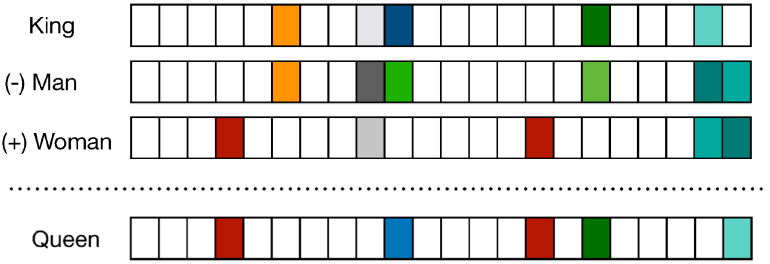
\includegraphics[width=\linewidth]{distributed_representation.png}
\subsection{Cosine-similarity or Cosine-distance}
\includegraphics[width=\linewidth]{cosine-similarity.jpg}